\documentclass[a4paper, 12pt]{report}
\usepackage[utf8]{inputenc} % symboler, såsom æøå eller lignende
\usepackage{textcomp} % flere symboler, såsom €
\usepackage{fontawesome}
\usepackage{graphicx} % Muliggør brug af figurer
\usepackage{float} % Muliggør positionering af figurer
\usepackage{wrapfig} % Muliggør tekst og figur på samme linje
\usepackage{caption}
\usepackage{subcaption} % Muliggør subfigures
\usepackage{hyperref} % interaktive referencer!
\usepackage{csquotes} % bruges af babel pakken
\usepackage[english]{babel} % rapportens sprog. Skal også rettes i "main.tex" under "\selectlanguage"
\usepackage[font = small, labelfont = bf]{caption} % til mindre figur tekster hvor figur nummeret er fremhævet med fed
\usepackage{xcolor} % Til brugerdefinerede farvekoder
\usepackage{mathptmx} % Til brugerdefinerede font størrelser
\usepackage{pdfpages} % for an kunne importere hele pdf sider
\usepackage{booktabs} % for at definere /toprule og /midrule
\usepackage{hyperref} %Muliggør brug af hyperref

% load a colour package
\usepackage{xcolor}
\definecolor{aaublue}{RGB}{33,26,82}% dark blue
\usepackage{graphicx} % Set up how figure and table captions are displayed

\usepackage[font = small, labelfont = bf]{caption} % til mindre figur tekster hvor figur nummeret er fremhævet med fed
\usepackage{xcolor} % Til brugerdefinerede farvekoder
\usepackage{mathptmx} % Til brugerdefinerede font størrelser
\usepackage{pdfpages} % for an kunne importere hele pdf sider
\usepackage{booktabs} % for at definere /toprule og /midrule
\usepackage{ulem} %math
\usepackage{amsmath} %Math
\usepackage{xcolor,colortbl} % farver i tabeller
\usepackage{multicol}%kolonner
\hyphenpenalty=100000 % *EKSPERIMENTIEL* Forhindrer automatisk deling af ord

% ------ Marginer ------
\usepackage[left = 2cm, right = 2cm, bottom = 3cm ,top = 3.5cm]{geometry} % juster selv marginerne ved at indtaste andre tal

% ------ Farver ------
\definecolor{chapterNumColor}{RGB}{150, 150, 150} % 255, 255, 255 er helt hvid. 0, 0, 0 er helt sort

% ------ Lister ------
% ducomentation for list options: http://www.texnia.com/archive/enumitem.pdf
\usepackage{enumitem} % til redigering af lister
\setlist{itemsep = 0.5cm, itemindent = 0cm, labelsep = 0.5cm, leftmargin = 0.5cm} % globale indstillinger for lister.

% ------ Referencer ------
% Biblatex cheat sheet: http://tug.ctan.org/info/biblatex-cheatsheet/biblatex-cheatsheet.pdf
\usepackage[backend=biber, style=numeric, sorting=none]{biblatex}
\appto{\bibsetup}{\raggedright}
\addbibresource{referencer.bib} % fortæller hvad vores reference bibliotek hedder og hvor det er at finde i mappestrukturen


%\DeclareFieldFormat{postnote}{s. #1} % ændrer "page" til "s." i kilder ved enkelte sider
%\DeclareFieldFormat{multipostnote}{s. #1} % ændrer "pages" til "s." i kilder ved interval af sider

% Sørger for at der står et al. når der er flere end to forfattere.
\DefineBibliographyStrings{danish}{
  andothers = {et\addabbrvspace al\adddot}
}

% ------ Indholdsfortegnelse (Table of contents (TOC)) ------
\usepackage{tocloft}
\setcounter{secnumdepth}{3} % jo højere tallet er, jo "dybere" overskrifter bliver nummereret. 3 giver Chapter, section, subsection og subsubsection
\setcounter{tocdepth}{2} % dybden af indholdfortegnelsen. 1 viser chapter, section og sub
% \renewcommand{\cftpartleader}{\cftdotfill{\cftdotsep}} % prikker for parts
% \renewcommand{\cftchapleader}{\cftdotfill{\cftdotsep}} % prikker for chapters
% \renewcommand{\cftsecleader}{\hfill} % fjern prikker for sections
% \renewcommand{\cftsubsecleader}{\hfill} % prikker for subsections

% ------ Sidehoved og sidefod ------
\usepackage{lastpage} % Gør det muligt at få vist sidenummer for sidste side i rapporten.
\usepackage{fancyhdr} % Pakke til at modificere sidehoved og sidefod
\fancyhf{} % Sætter header og footer til ikke at indeholde noget - så vi er klar til at give det nyt indhold
\setlength{\headheight}{15pt} % Bestemmer hvor langt nede sidehovedet vises
\fancyfoot[R]{\thepage \ af \pageref{LastPage}} % Viser sidenummeret nederst til højre. Ændr "R" for at få det placeret et nyt sted
\fancyhead[L]{\leftmark} % placerer sidehoved indhold i øverste venstre side

\fancypagestyle{plain} % Brugerdefineret side når styletypen plain er valgt. I dette tilfælde er det hver gang et kapitel opstår. 
{
    \fancyhf{} % Sætter header og footer til ikke at indeholde noget - så vi er klar til at give det nyt indhold
    \renewcommand{\headrulewidth}{0pt} % Fjerner linjen øverst under sidehovedet
    \fancyfoot[R]{\thepage \ af \pageref{LastPage}} % Viser sidenummeret nederst til højre. Ændr "R" for at få det placeret et nyt sted
}
\pagestyle{fancy}

% ------ Style for kapitlers sidehoved ------
\usepackage{titlesec} % Til brugerdefinerede sidehoved
\titleformat{\chapter}{\fontsize{25pt}{25pt}\bfseries\color{black}}{{\color{chapterNumColor}\thechapter}}{15pt}{} % sætter fonttypen, skriftstørrelsen og farven på kapitel
\titlespacing*{\chapter}{0pt}{-50pt}{40pt} %Kapitelhøjde
\titleformat{\part}{\fontsize{40pt}{45pt}\bfseries\centering\color{black}}{{\color{chapterNumColor}\thepart}}{15pt}{}[\thispagestyle{empty}\addtocounter{page}{-1}] % sætter fonttypen, skriftstørrelsen og farven på parts

% ------ Selvlavede kommandoer til citater ------

\newcommand{\centerQuote}[3] % Indholdet i {} er navnet på den kommando der er lavet
{
    \begin{quote} % Sørger for at centrere dit citat
        \textit{"#1"} - \parencite[#2]{#3} % Laver formatet "Citat her" - (Efternavn, Årstal, s. sidetal)
    \end{quote} 
}

\newcommand{\inlineQuote}[3] % Indholdet i {} er navnet på den kommando der er lavet
{\textit{"#1"} \parencite[#2]{#3}} % Laver formatet "Citat her" - (Efternavn, Årstal, s. sidetal)

\usepackage{lipsum} % til at generere dummy text. Brug \lipsum[2] for at vise paragraf nr 2 i Lorem Ipsum. Brug \lipsum[4-7] for at vise paragraf 4 til 7 i Lorem Ipsum.

% ------ ToDo Notes ------
%ToDo Notes cheat sheet: https://mirrors.dotsrc.org/ctan/macros/latex/contrib/todonotes/todonotes.pdf
\setlength{\marginparwidth}{2cm} % Retter fejl med marginer i ToDo notes.
\usepackage{todonotes} % Muliggør brug af "ToDo notes" funktionalliteter

%------ Glossary ------
%Glossaries cheat sheet: https://mirrors.dotsrc.org/ctan/macros/latex/contrib/glossaries/glossariesbegin.pdf
\usepackage{glossaries} % Muliggør brug af "glossaries funktionen"
\makenoidxglossaries % Muliggør udskift af glossary-list i dokumentet
\glstoctrue % Inkluderer glossary i toc
\setacronymstyle{long-short}

% Place is in alphabetical order, first letter only needs to be in order. !

\newacronym{axo}{AXO}{abandoned explosive ordnance}
\newacronym{cmc}{CMC}{cluster munition coalition}
\newacronym{erw}{ERW}{explosive remnants of war}
\newacronym{icbl}{ICBL}{International Campaign to Ban Landmines}
\newacronym{icrc}{ICRC}{International Committee of the Red Cross}
\newacronym{lm}{LM}{Landmine Monitor}
\newacronym{ngo}{NGO}{non-governmental organization}
\newacronym{svm}{SVM}{support vector machine}
\newacronym{unmas}{UNMAS}{United Nations Mine Action Service} 
\newacronym{un}{UN}{United Nations}
\newacronym{uxo}{UXO}{unexploded ordnance}
\newacronym{sota}{SOTA}{state-of-the-art}
\newacronym{at}{AT}{Anti-Tank}
\newacronym{ap}{AP}{Anti-Personnel}
\newacronym{gpr}{GPR}{Ground Penetrating Radar}
 % Muliggør brug af glossary.tex for samlede definitioner


%------ Boxes -------
\newlength{\mylen}
\settowidth{\mylen}{text to}


%------- Timelines -------
\usepackage{chronology}

%------- Til at lave culonner -----
\usepackage{multicol}

%------- Til at vise program code -----
\usepackage{inconsolata}
\usepackage{listings}
\lstset { %
    language=C++,
    basicstyle=\ttfamily\small,
    numberstyle=\footnotesize,
    numbers=left,
    backgroundcolor=\color{gray!10},
    frame=single,
    tabsize=2,
    rulecolor=\color{black!30},
    title=\lstname,
    escapeinside={\%*}{*)},
    breaklines=true,
    breakatwhitespace=true,
    framextopmargin=2pt,
    framexbottommargin=2pt,
	extendedchars=true,
    literate={å}{{\r{a}}}1 {ø}{{\o{}}}1 {á}{{\'a}}1 {ã}{{\~a}}1 {é}{{\'e}}1,
    %inputencoding=utf8
}

%------- Requirements table -------
\newcolumntype{L}[1]{>{\raggedright\let\newline\\\arraybackslash\hspace{0pt}}m{#1}}
\newcolumntype{C}[1]{>{\centering\let\newline\\\arraybackslash\hspace{0pt}}m{#1}}
\newcolumntype{R}[1]{>{\raggedleft\let\newline\\\arraybackslash\hspace{0pt}}m{#1}}
\usepackage{longtable, array}
% \setlength\extrarowheight{0pt}
% \setlength{\arrayrulewidth}{0.3mm}
\renewcommand{\arraystretch}{1.5}
\usepackage{makecell}
\usepackage{mwe}


% ------ Strike through text --------
\usepackage{soul}


%------- Bash color coding ----------
\lstset{ 
    language=bash, % choose the language of the code
    basicstyle=\fontfamily{pcr}\selectfont\footnotesize\color{black},
    keywordstyle=\color{black}\bfseries, % style for keywords
    numbers=left, % where to put the line-numbers
    numberstyle=\tiny, % the size of the fonts that are used for the line-numbers
    showspaces=false, % show spaces adding particular underscores
    showstringspaces=false, % underline spaces within strings
    showtabs=false, % show tabs within strings adding particular underscores
    frame=single, % adds a frame around the code
    tabsize=2, % sets default tabsize to 2 spaces
    rulesepcolor=\color{gray},
    rulecolor=\color{black},
    captionpos=b, % sets the caption-position to bottom
    breaklines=true, % sets automatic line breaking
    breakatwhitespace=false, 
    emph={rosrun,int,char,double,float,unsigned,void,bool},
    emphstyle={\color{blue!50}},
}

%---------- Ditto mark---------

\usepackage{tikz}
\newcommand{\dittotikz}{%
    \tikz{
        \draw [line width=0.12ex] (-0.2ex,0) -- +(0,0.8ex)
            (0.2ex,0) -- +(0,0.8ex);
        \draw [line width=0.08ex] (-0.6ex,0.4ex) -- +(-1.5em,0)
            (0.6ex,0.4ex) -- +(1.5em,0);
    }%
}

%----------- For having recurring text in the report to show the same ----------

\usepackage{clipboard}

%%%%%%%%%%%%%%%%%%%%%%%%%%%%%%%%%%%%%%%%%%%%%%%%
% Macros for the title page
%%%%%%%%%%%%%%%%%%%%%%%%%%%%%%%%%%%%%%%%%%%%%%%%
%Creates the aau title page
\newcommand{\aautitlepage}[3]{%
  {
    %set up various length
    \ifx\titlepageleftcolumnwidth\undefined
      \newlength{\titlepageleftcolumnwidth}
      \newlength{\titlepagerightcolumnwidth}
    \fi
    \setlength{\titlepageleftcolumnwidth}{0.5\textwidth-\tabcolsep}
    \setlength{\titlepagerightcolumnwidth}{\textwidth-2\tabcolsep-\titlepageleftcolumnwidth}
    %create title page
    \thispagestyle{empty}
    \noindent%
    \begin{tabular}{@{}ll@{}}
      \parbox{\titlepageleftcolumnwidth}{
        \iflanguage{danish}{%
          
\includegraphics[width=\titlepageleftcolumnwidth]{00 - Images/aau_logo_da.pdf}
        }{%
          
\includegraphics[width=\titlepageleftcolumnwidth]{00 - Images/aau_logo_en.pdf}
        }
      } &
      \parbox{\titlepagerightcolumnwidth}{\raggedleft\sf\small
        #2
      }\bigskip\\
       #1 &
      \parbox[t]{\titlepagerightcolumnwidth}{%
      \textbf{Abstract:}\bigskip\par
        \fbox{\parbox{\titlepagerightcolumnwidth-2\fboxsep-2\fboxrule}{%
          #3
        }}
      }\\
    \end{tabular}
    \vfill
    \iflanguage{danish}{%
      \noindent{\footnotesize\emph{Rapportens indhold er frit tilgængeligt, men offentliggørelse (med kildeangivelse) må kun ske efter aftale med forfatterne.}}
    }{%
      \noindent{\footnotesize\emph{The content of this report is freely available, but publication (with reference) may only be pursued due to agreement with the author.}}
    }
    \clearpage
  }
}

%Create English project info
\newcommand{\englishprojectinfo}[8]{%
  \parbox[t]{\titlepageleftcolumnwidth}{
    \textbf{Title:}\\ #1\bigskip\par
    \textbf{Theme:}\\ #2\bigskip\par
    \textbf{Project Period:}\\ #3\bigskip\par
    \textbf{Project Group:}\\ #4\bigskip\par
    \textbf{Participant(s):}\\ #5\bigskip\par
    \textbf{Supervisor(s):}\\ #6\bigskip\par
    \textbf{Copies:} #7\bigskip\par
    \textbf{Page Numbers:} \pageref{LastPage}\bigskip\par
    \textbf{Date of Completion:}\\ #8
  }
}

%Create Danish project info
\newcommand{\danishprojectinfo}[8]{%
  \parbox[t]{\titlepageleftcolumnwidth}{
    \textbf{Titel:}\\ #1\bigskip\par
    \textbf{Tema:}\\ #2\bigskip\par
    \textbf{Projektperiode:}\\ #3\bigskip\par
    \textbf{Projektgruppe:}\\ #4\bigskip\par
    \textbf{Deltager(e):}\\ #5\bigskip\par
    \textbf{Vejleder(e):}\\ #6\bigskip\par
    \textbf{Oplagstal:} #7\bigskip\par
    \textbf{Sidetal:} \pageref{LastPage}\bigskip\par
    \textbf{Afleveringsdato:}\\ #8
  }
}

\begin{document}
%% FRONT MATTER
\fontfamily{ptm}\selectfont % times font
\pagenumbering{Roman} %use roman page numbering in the frontmatter

%  A simple AAU report template.
%  2015-05-08 v. 1.2.0
%  Copyright 2010-2015 by Jesper Kjær Nielsen <jkn@es.aau.dk>
%
%  This is free software: you can redistribute it and/or modify
%  it under the terms of the GNU General Public License as published by
%  the Free Software Foundation, either version 3 of the License, or
%  (at your option) any later version.
%
%  This is distributed in the hope that it will be useful,
%  but WITHOUT ANY WARRANTY; without even the implied warranty of
%  MERCHANTABILITY or FITNESS FOR A PARTICULAR PURPOSE.  See the
%  GNU General Public License for more details.
%
%  You can find the GNU General Public License at <http://www.gnu.org/licenses/>.
%
\pdfbookmark[0]{Front page}{label:frontpage}%
\begin{titlepage}
  \addtolength{\hoffset}{0.5\evensidemargin-0.5\oddsidemargin} %set equal margins on the frontpage - remove this line if you want default margins
  \noindent%
  \begin{tabular}{@{}p{\textwidth}@{}}
    \toprule[2pt]
    \midrule
    \vspace{0.2cm}
    \begin{center}
    \Huge{\textbf{
      P1 Project% insert your title here
    }}
    \end{center}
    \begin{center}
      \Large{
        - Mobile Robot for Localization of Landmines -% insert your subtitle here
      }
    \end{center}
    \vspace{0.2cm}\\
    \midrule
    \toprule[2pt]
  \end{tabular}
  \vspace{4 cm}
  \begin{center}
    {\large
      Made by%Insert document type (e.g., Project Report)
    }\\
    \vspace{0.2cm}
    {\Large
      ROB1 B332-b%Insert your group name or real names here
    }
  \end{center}
  \vfill
  \begin{center}
  Aalborg University\\
    The Technological Faculty for IT and Design\\
    Department of Electronic Systems
  \end{center}
\end{titlepage}
\clearpage % forside

\cleardoublepage

\addcontentsline{toc}{chapter}{Title page}
\thispagestyle{empty}
\pdfbookmark[0]{English title page}{label:titlepage_en}
\aautitlepage{%
  \englishprojectinfo{
    Mobile robots used in Humanitarian demining %title
  }{%
    Reality and models %theme
  }{%
    ROB1 P1 1st Semester %project period
  }{%
    B332 % project group
  }{%
    %list of group members
    Jesper Poscholann Hammer\\
    Maiken Cecilie Lanng\\
    Kjartan Nolsøe Jespersen\\ 
    Kasper Maarschalk Hytting
  }{%
    %list of supervisors
    Matthias Rehm
  }{%
    1 % number of printed copies
  }{%
    \today % date of completion
  }%
}{%department and address
  \textbf{The Technological Faculty for IT and Design}\\
  Department of electronic systems\\
  Niels Jernes Vej 10, 9220 Aalborg Øst\\
  \href{http://www.aau.dk}{http://www.aau.dk}
}{% the abstract
Landmines are a major risk to civilian populations in affected areas. It is estimated that 59 countries still are influenced by landmines and other explosives. This provides a financial burden for governments and a health risk for the population in the proximity of these mine areas.

The report sheds light on the devastating amount of casualties due to landmines trough out the world and it is soon revealed that Afghanistan has the highest death count, hence this report will have a slight focus on that country.\\
    
The process of finding and removing landmines is called demining. This report mainly focuses on humanitarian demining, because of the needed assistance in making this easier, safer, and faster. Current humanitarian demining is a dangerous endeavor and therefore development in robotics to assist in demining is being made. These robots vary a lot in their specifications and are still not properly implemented in the demining process. This could be because of the cost, the robots’ specialization in singular types of mines, or the advanced systems and mechanics. Some of the current robots will be presented in this report.
}  % titelside (EN)
\chapter*{Preface\markboth{Preface}{Preface}}\label{ch:preface}
\addcontentsline{toc}{chapter}{Preface}
\thispagestyle{empty}

This project has been interesting in the way that it taught me to work with ROS programming to the extent that I could see what Robotics Engineering is all about, peace out.
\begin{flushright}
- KNJ
\end{flushright}
\todo{We can write something personal here, our own ideas or learnings from the project, before we submit the report}

\vspace{\fill}

\textit{Signatures:}

\vspace{3\baselineskip}

\vspace{1mm}

\begin{minipage}[b]{0.45\textwidth}
 \centering
 \rule{\textwidth}{0.5pt}\\
  {\footnotesize Jesper Poscholann Hammer}\\
 {\footnotesize jhamme19@student.aau.dk}
\end{minipage}
\hfill
\begin{minipage}[b]{0.45\textwidth}
 \centering
 \rule{\textwidth}{0.5pt}\\
  {\footnotesize Maiken Cecilie Lanng}\\
 {\footnotesize mlanng19@student.aau.dk}
\end{minipage}
\vspace{3\baselineskip}

\vspace{1mm}

\begin{minipage}[b]{0.45\textwidth}
 \centering
 \rule{\textwidth}{0.5pt}\\
  {\footnotesize Kjartan Nolsøe Jespersen}\\
 {\footnotesize knje20@student.aau.dk}
\end{minipage}
\hfill
\begin{minipage}[b]{0.45\textwidth}
 \centering
 \rule{\textwidth}{0.5pt}
 {\footnotesize Kasper Maarschalk Hytting}\\
 {\footnotesize khytti19@student.aau.dk}
\end{minipage}

    
\newpage
087
\selectlanguage{english} %Skal også rettes i "preample.tex" under "\usepackage[danish, english]"
%%%%%

%% Contents
\tableofcontents
\thispagestyle{empty}
\cleardoublepage
%\listoftodos
%%%%%

%% MAIN MATTER
\pagestyle{fancy}
\pagenumbering{arabic} %use arabic page numbering in the mainmatter
%%%%%

%% INPUT HERUNDER
\chapter{Introduction} \label{chap:Introduction}

Landmine are encased explosive charges either buried just below the surface of the ground, buried deep under ground, or placed above ground hidden in bushes, grass, etc.\\
Landmines generally have more or less simple trigger mechanisms, such as \cite{EB:Mine}:

\begin{itemize}
\setlength{\itemsep}{0.05\baselineskip}
    \item Pressure censors; reacting when weight of persons, vehicles, cattle, etc. exceeds a preset limit
    \item Tripwires; reacting when the wire is pulled or stepped on
    \item Remote control; manually detonating the mine from a remote position
    \item Timers; detonating the mine after a preset amount of time
\end{itemize}

The versatility and simplicity of landmines in combination with the strategic advantage of being able to effect the enemy, without tying own troops in the operation has made landmines a popular weapon to use in times of conflict and war throughout history.

Landmines are cheap to manufacture, and therefore they have been produced and deployed in great numbers since their invention. As a result, many active mines remain buried/hidden throughout the world. Presently, it is estimated that 59 countries are still affected by landmines.

However, statistics also show that the work done throughout the past 20 years has resulted in 2880 square kilometres of land being cleared of landmines, and more than 4,6 million anti-personnel mines being destroyed. It is estimated that there are more than 2000 square kilometres of landmine contaminated land remaining thru out the world \cite{clearingTheMines}.\\

The purpose of landmines range from preventing an opponent access to critical installations or areas of strategic value, to leading the enemy a specific way on the battlefield, to simply instilling fear and demoralizing the enemy. Furthermore the minefield, also functions as an alarm system, because of the loud noise created by the explosions \cite{clearingTheMines}.\\

A heavy downside to mines is that they do not distinguish between military opponents, civilians or even animals.

This means that the usefulness of mines in times of war turns into a problem for the country and especially its population in the aftermath of the war. Landmines restrict access to parts of the country and limit the the population in utilizing agricultural land, roads, etc.

Landmines further effect the population, as many civilians fall victim to them each day - ether suffering death or serious injuries such as dismemberment or organ damages caused by fragments  \cite{clearingTheMines}\\.

Over 20 years ago countries started a joint effort to rid the world of landmines. This involved putting more focus on the issue and laying in the financial resources needed to start the work of locating and destroying the landmines, which is also known as demining \cite{clearingTheMines}.

This joint effort is known as the Ottawa Convention, or formally: the Anti-Personnel Mine Ban Treaty. The treaty was drafted under the UN in 1997 and put into motion in 1999 \cite{treatyICBL}.\\

\noindent The International Mine Action Standards, also known as IMAS, defines demining as such:\\

“\textit{Activities which lead to the removal of Explosive Ordnance hazards, including technical survey, mapping, clearance, marking, post-clearance documentation, community mine action liaison and the handover of cleared land. Demining may be carried out by different types of organizations, such as NGOs, commercial companies, national mine action teams or military units. Demining may be emergency-based or developmental.}” \cite{IMAS}\\

\noindent IMAS also states that humanitarian demining and demining are interchangeable terms \cite{IMAS}.\\

Demining still relies heavily on manual labour, which is very time demanding and involves a big risk of injury to the workers.

However, over the years a lot of advances have been made to speed up this process and reduce the risk to the workers. Some of these include heavy reinforced vehicles capable of withstanding explosions, intended to simply trigger the landmines by various mechanisms.

More recently these advances has had an increasing focus on semi-automated and fully automated systems, presently leading to the development of demining robots. Demining robots such as the MineWolf have been developed in order to remove mines in a way, that limits or excludes the human involvement in the direct detection and removal of the mines \cite{mineWolf}.

\setlength{\parindent}{0pt}
\chapter{Casualties} \label{chap:casualties}

Currently, a large part of the world is contaminated by mines and ERW as seen in figure \textbf{\ref{fig:contamination_mine_erw}}, this affects a large number of people in their day to day life. Landmines do not discriminate. Thus victims can be men, women, children, people from all nationalities, and ages. Hence as mentioned in the introduction, the Anti-Personnel Mine Ban Treaty was introduced in 1999, which has lead to yearly rising contributions from the state parties ever since. \cite{LandmineMonitor2019} 

        \vspace{5mm}

\begin{centering}

\textit{\large “A landmine is the perfect soldier: Ever courageous, never sleeps, never misses"}\\

\begin{flushright}

        \vspace{-3mm}
        
-- Paul Jefferson, one of the earliest humanitarian deminers \hspace{4mm}

\end{flushright}
\end{centering}

%%%

\section{Casualties in Numbers}

% First use: \gls{svm}. Second use: \gls{svm}.

The landmine monitor 2019 is a report formed by the \gls{icbl} and the \gls{cmc}, the data in the report is processed by the Monitoring and Research Committee, a standing committee of the ICBL-CMC Governance Board. Which is comprised of five \gls{ngo}s, as well as Monitor research team leaders and ICBL-CMC staff and contributions from 11 countries. All of them contributing to writing the annual landmine monitoring report. Furthermore, the landmine monitor is approved and provided by the \gls{un} \cite{LandmineMonitor2019}.

        \vspace{2mm}

\begin{figure}[!ht]
  \centering
  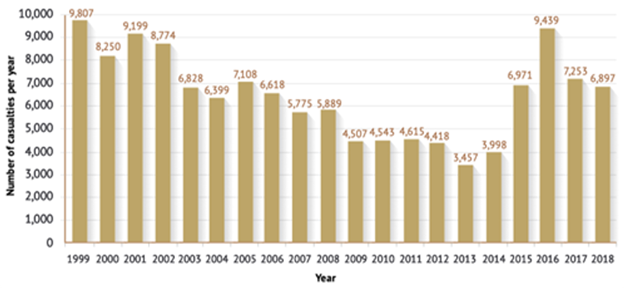
\includegraphics[width=12.5cm]{00 - Images/casualties_per_year.png}
  \caption{Casualties annually due to landmines/\gls{erw} (1999-2018) \cite{LandmineMonitor2019}}
  \label{fig:casualties_per_year}
\end{figure}

\newpage

An increase in conflicts and wars in 2014-16, entails a big spike in the global number of casualties by landmines, as seen in Figure \ref{fig:casualties_per_year}. These casualties come from two main categories of explosive war remains: The standard landmines and the \gls{erw}, which covers the \gls{uxo}. UXOs include weapons that failed to detonate and \gls{axo}. AXOs are weapons that have never been used in conflicts and were abandoned by the party that owned it \cite{Remnants2019:online}. 

        \vspace{2mm}

As a result of the Mine Ban Treaty, the people who still use these banned explosives turned to make homemade and improvised mines, which is why most mines are of this kind today. This causes a lot of problems, because of the variety in design and internal contents of the mines, which makes it difficult to remove and destroy them. This is due to a lack of knowledge of the construction of the mines. The lack of reporting to the authorities, when an improvised mine is planted, entails many unrecorded casualties. In 2009-2014 where the global landmine casualties were at its lowest, it was estimated that there was annually between 700 and 1300 extra casualties, which is not included in these statistics. 

        \vspace{2mm}

Since the mine ban treaty was initially introduced, back in 1999, there have been recorded 130.745 casualties. The total sum of casualties in different countries is still rising every day, the 2019 report states that; the estimated number of casualties per day worldwide is 18 during the 19-year period from 1999-2018 \cite{LandmineMonitor2019}.

        \vspace{2mm}

\begin{wrapfigure}[15]{r}{0.50\textwidth}
    \vspace{-5mm}
    \centering
      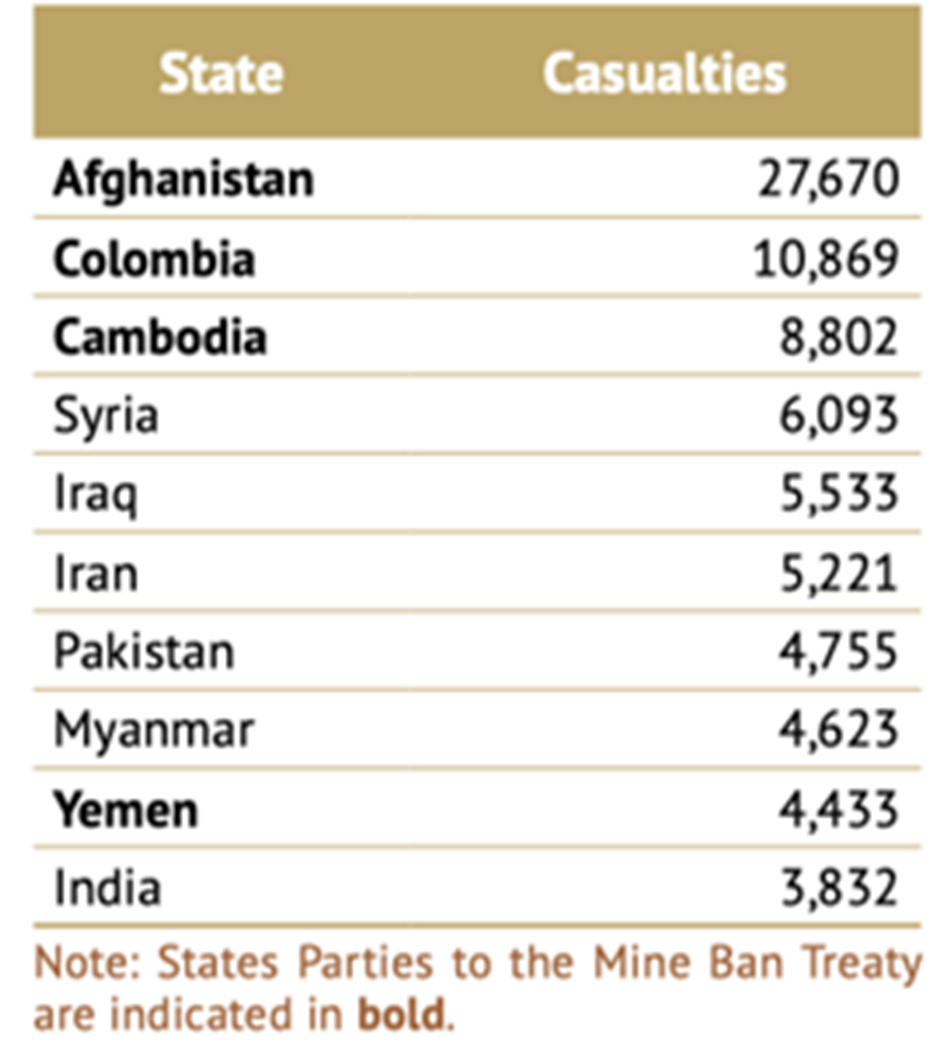
\includegraphics[width=0.45\textwidth]{00 - Images/casualties_per_country.png}
  \caption{Countries with the highest total casualties (1999 – 2018) \cite{LandmineMonitor2019}}
  \label{fig:casualties_per_country}
\end{wrapfigure}

Figure \ref{fig:casualties_per_country} states the countries with the highest total casualties from 1999-2018 caused by mines/\gls{erw}, were countries such as Afghanistan, Colombia, and Cambodia had a death count of 47.341 people - this corresponds to 36,2\% of the total casualties during this period. These countries are or were experiencing conflicts and are members of the mine ban treaty, which implies that these countries have a higher number of improvised mines. This results in increased difficulty in removing the landmines. Furthermore, the listed countries have very different environments that raise yet another problem, and a need for a problem limitation, or a universal solution which can locate mines in all kinds of terrain \cite{LandmineMonitor2019}.

\clearpage

\section{Casualty Demographics}
Statistics show that there were at least 1.714 child\footnote{Child casualties are defined as all casualties where the victim is less than 18 years of age at the time of the incident.} casualties in 2018 caused by mines/\gls{erw}. The child casualties made up 40\% of all the casualties where the age was known. The statistics distinguish the sex of the children, showing that the vast majority corresponding to 84\% are boys.

        \vspace{2mm}

A broad look at the statistics from 2018 men and boys made up 88\% of the casualties, whereas women and girls made up the remaining 12\% of all casualties where the sex was known. Civilians represented 71\% of casualties where the status\footnote{The status ranges between military, civilian, deminer} was known - these casualties were recorded in 38 states in different areas \cite{LandmineMonitor2019}.

\section{Casualties by Mine Type}

In 2018, mines caused at least 4.885 casualties in total. These can be split up into four groups: 
\begin{itemize}
    \item Antipersonnel mines
            \vspace{-4mm}
    \item Anti-vehicle mines
            \vspace{-4mm}
    \item Improvised mines
            \vspace{-4mm}
    \item Other unspecified mines
\end{itemize}

The deadliest type of mine is the improvised mine, causing 3.789 casualties, which is the largest part of the total casualties registered, as seen in Figure \ref{fig:casualties_by_type}. Out of the 3.789 casualties, it was recorded that 1.752 (46\%) of these casualties were identified to be specifically improvised, antipersonnel mines. \gls{erw} does also have a large place in the statistics, causing 1.410 casualties \cite{LandmineMonitor2019}.

\begin{figure}[!ht]
  \centering
  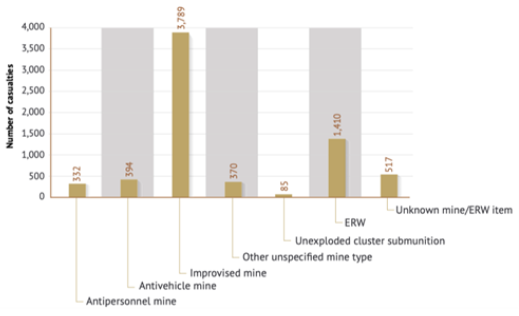
\includegraphics[width=12.5cm]{00 - Images/casualties_by_type.png}
  \caption{Casualties by type of mine/\gls{erw} in 2018 \cite{LandmineMonitor2019}}
  \label{fig:casualties_by_type}
\end{figure}
\chapter{The Focus on the Problem}

\section{The History}

As one can see from the following list:
\begin{itemize}
\setlength{\itemsep}{0.05\baselineskip}
    \item Journals of the Continental Congress - Articles of War, 20 September, 1776 . \cite{ArticlesOfWar1775:online}\\
    \textit{An example: Section XIII, Article 12: Whatsoever officer or soldier shall misbehave himself before the enemy, or shamefully abandon any post committed to his charge, or shall speak words inducing others to do the like, shall super death.}
    \item General Orders No. 100 : The Lieber Code, Instuctions for the government of armies of the US in the field, 24 April 1863. \cite{LiberCode1863:online}\\
    \textit{An example: Article 16: Military necessity does not admit of cruelty - that is, the infliction of suffering for the sake of suffering or for revenge, nor of maiming or wounding except in fight, nor of torture to extort confessions. It does not admit of the use of poison in any way, nor of the wanton devastation of a district. It admits of deception, but disclaims acts of perfidy; and, in general, military necessity does not include any act of hostility which makes the return to peace unnecessarily difficult. }
    \item Amelioration of the Condition of the Wounded on the Field of Battle (Red Cross Convention), First Geneva Convention; 22 August, 1864. \cite{1stGenevaConvention1864:online}\\
    \textit{An example: Article 1: Ambulances and military hospitals shall be acknowledged to be neuter, and, as such, shall be protected and respected by belligerents so long as any sick or wounded may be therein.\\
    Such neutrality shall cease if the ambulances or hospitals should be held by a military force. }
    \item Final Act of the Diplomatic Conference of Geneva, 12 August 1949. \cite{FinalGenevaConvention1949:online}\\
    \textit{An example: ARTICLE 34: During the last two world wars, hostages were imprisoned, often put in solitary confinement, deported and in many cases executed without previous warning or trial.\\
    The International Committee of the Red Cross considered that the prohibition of such practices, which are based on contempt for the principle of individual responsibility for breaches of the law, must be one of the essential elements in the new Convention.}
\end{itemize}
Changes to the conduct of warfare by nations, and on a global scale, has been put in place. These conducts have also been updated to also contain articles enforcing practices , as Prof. Yves Sandoz writes, "for the protection of persons at the mercy of or in the hands of their enemy" and practices to prevent "Use of certain conventional weapons which may be deemed to be excessively injurious or to have indiscriminate effects" \cite{ConventionalWeapons1980:online}\\

\iffalse
\begin{chronology}[3]{1991}{2012}{\linewidth}[17cm]
\event{\decimaldate{}{9}{1991}}{{“The Coward’s War: Landmines in Cambodia" report}}
\event{\decimaldate{}{10}{1992}}{{Six \gls{ngo}s meet and agree to coordinate campaigning efforts}}
\event{\decimaldate{}{5}{1993}}{{The ICBL holds its First International \gls{ngo} Conference on Landmines}}
\event{\decimaldate{}{3}{1994}}{{UNICEF Director Jim Grant calls for a landmine ban}}
\event{\decimaldate{}{3}{1995}}{{Belgium becomes the first country to pass a national law banning landmine}}
\event{\decimaldate{}{10}{1996}}{{Canada hosts a conference in Ottawa attended by 75 governments, the ICBL and international agencies}}
%\event{\decimaldate{}{10}{1997}}{{The ICBL and Jody Williams are awarded the Nobel Peace Prize for their crucial roles}}
\event{\decimaldate{}{11}{1997}}{{A total of 122 nations sign the Mine Ban Treaty in Ottawa, Canada}}
\event{\decimaldate{}{6}{1998}}{{The ICBL creates the Landmine Monitor initiative to verify nations’ compliance with the Mine Ban Treaty}}
\event{\decimaldate{}{3}{1999}}{{Mine Ban Treaty enters into force on 1 March 1999, becoming binding international law}}
\event{\decimaldate{}{7}{2000}}{{Mauritania becomes the 100Th country to ratify the Mine Ban Treaty}}
\event{\decimaldate{}{3}{2003}}{{All States Parties with stockpiles to destroy complete their obligations deadline.}}
\event{\decimaldate{}{9}{2004}}{{An international symposium on the challenges of achieving a mine-free world is held in Ottawa.}}
\event{\decimaldate{}{10}{2012}}{{The ICBL celebrates its 20Th anniversary}}
\end{chronology}
\fi

\begin{figure}[ht!]
    \begin{chronology}[3]{1991}{2013}{\linewidth}[17cm]
\event{\decimaldate{}{}{1991}}{{\gls{ngo}s supporting a ban on landmines begin collaborating.}}
\event{\decimaldate{}{}{1992}}{{International campaign to ban landmines is established.}}
\event{\decimaldate{}{}{1993}}{{First international meeting of NGOs held in London.}}
\event{\decimaldate{}{}{1994}}{{ICRC declares its support for a ban on antipersonnel landmines.}}
\event{\decimaldate{}{}{1995}}{{First national law banning antipersonnel mines.}}
\event{\decimaldate{}{}{1996}}{{Canada launches the Ottawa process to ban landmines.}}
%\event{\decimaldate{}{10}{1997}}{{The ICBL and Jody Williams are awarded the Nobel Peace Prize for their crucial roles}}
\event{\decimaldate{}{}{1997}}{{Mine Band Treaty adopted  and opened for signature.}}
\event{\decimaldate{}{}{1998}}{{Mine Ban Treaty's 40Th ratification is secured in record time.}}
\event{\decimaldate{}{}{1999}}{{The Mine Ban Treaty becomes international law.}}
\event{\decimaldate{}{}{2000}}{{Mine Ban Treaty reaches 100 states parties.}}
\event{\decimaldate{}{}{2002}}{{Affected states continue to join the Mine Ban Treaty.}}
\event{\decimaldate{}{}{2003}}{{First Stockpile destruction - Deadlines are met.}}
\event{\decimaldate{}{}{2004}}{{First Review conference of the Mine Ban Treaty.}}
event{\decimaldate{}{}{2005}}{{Use of landmines decreases.}}
\event{\decimaldate{}{}{2006}}{{Act Now to implement the Mine Ban Treaty.}}
\event{\decimaldate{}{}{2007}}{{A Success in Progress: The Mine Ban Treaty's first decade.}}
\event{\decimaldate{}{}{2009}}{{“Mission Possible” – Mine Ban Treaty's second review conference.}}
\event{\decimaldate{}{}{2010}}{{The United States consults on its landmine policy review.}}
\event{\decimaldate{}{10}{2012}}{{The ICBL-CMC celebrates its 20Th anniversary.}}
\end{chronology}
\caption{Timeline of the international campaign to ban landmines \cite{TimelineICBL:online}}
\label{fig:Timeline of the international campaign to ban landmines}
\end{figure}

\noindent Looking through the figure \ref{fig:Timeline of the international campaign to ban landmines} above, the \gls{ngo}s started in 1991 to address the issues with landmines with a report, Coward’s War - Land Mines in Cambodia, where in the report it was stated that the landmines resulted in devastating medical, social and psychological effects for Cambodia. \cite{Cambodia1991:online}. As one part in warfare, landmines have been used, but they state problems for the local civilians in the contaminated areas, see chapter \ref{chap:casualties}. And up until 1999 there was not any international law, enforced by the union of countries, to prevent countries at war to use landmines, but in 1999 the Mine Ban Treaty, also known as the Ottawa Treaty, became an international binding law that from 2000 was enforced by 100 countries, also referred to, on figure \ref{fig:Timeline of the international campaign to ban landmines}, as state parties. While this report was written, the Mine Ban Treaty is still being monitored by the \gls{icbl}. Publishing yearly the Landmine Monitor report. \cite{LandmineMonitor2019}


\section{UN's Involvement}

In 1997 the United Nations formed an initiative know as \gls{unmas} (Abbreviated \gls{unmas}), \gls{unmas} leads, coordinates and implements UN's demining efforts and to eliminate explosive hazards, according to UN the initiative has already saved lives and protected the livelihood of many civilians in areas of Libya, Colombia, Somalia, and many more
Further more \gls{unmas} provides some guidelines on how to give support to the survivors of landmines, although the support is mainly the responsibility of each state, but \gls{unmas} does say that all survivors should be treated fairly, which means the survivors should be treated neutrally and without discrimination

\newpage

\section{The Financial Aid for the Cause}

According to the \gls{icbl} \gls{lm} 2018. The total support for Mine Action in 2018 was US\$699.5. The funding for Min Action, mentioned in chapter \ref{chap:Introduction}, goes into different sections within the umbrella term Mine Action. The \gls{icbl} has set the sections as in the following figure \ref{fig:contributions_by_thematic_sector_2018}:

\begin{figure}[ht]
  \centering
  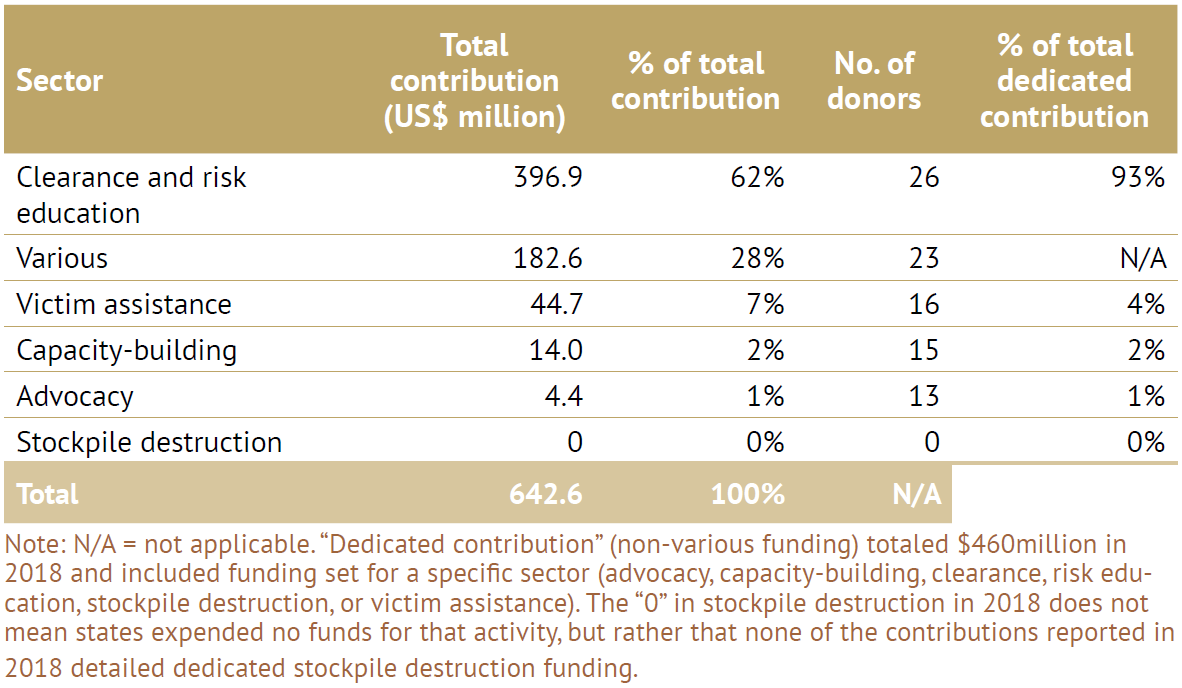
\includegraphics[width=0.6\linewidth]{00 - Images/contributions_by_thematic_sector_2018.png}
  \caption{Contributions by thematic sector 2018 \cite{LandmineMonitor2019}}
  \label{fig:contributions_by_thematic_sector_2018}
\end{figure}

The descriptiveness follows, mostly taken from \gls{lm}: 
\begin{itemize}
\setlength{\itemsep}{0.05\baselineskip}
    \item Clearance and risk education\\
    \textit{\textbf{Clearance} – Tasks or actions to ensure the removal and/or the destruction of all mine and ERW hazards from a specified area to a specified depth\\
    \textbf{Mine/\gls{erw} risk education} – Activities which seek to reduce the risk of injury from mines and  ERW by awareness-raising and  promoting behavioral  change, including public information dissemination, education and training, and community mine action liaison}
    \item Various\\
    \textit{Expenses that are not, or have not been, categorised into the other areas.}
    \item Victim assistance\\
    \textit{Victim assistance includes, but is not limited to, data collection and needs assessment, emergency and continuing medical care, physical rehabilitation, psychological support and social inclusion, economic inclusion, and laws and public policies to ensure the full and equal integration and participation of survivors, their families, and communities in society.}
    \item Capacity-building\\
    \textit{At the individual and organizational level, the focus is on increasing the availability of information and participation of underprivileged, underserved, or impoverished members of society. The purpose of these activities is to give voice and status to previously underrepresented populations. The mechanisms for building individual capacity are often leadership training, political activism, and community development. Programs that build awareness are also often highlighted. For nonprofit organizations and communities, capacity is built through technical assistance, organizational development, and interorganizational collaboration \cite{EB:capacity-building}.}
    \item Advocacy\\
    \textit{The most important assets at the disposal of advocacy networks are information and communication. Information is deployed to change actors’ perceptions and preferences and ultimately their behaviours. Information is invariably a critical component of conventional and unconventional campaign tactics, including education and capacity building, public relations, petitions, lobbying, and product or producer boycotts\cite{EB:advocacy-networking}.}
    \item Stockpile destruction\\
    \textit{Destruction of stockpiled anti-personnel mines}
\end{itemize}
\chapter{Mines and Specifications}

\section{What is a landmine}

\begin{wrapfigure}{R}{0.47\linewidth}
\centering
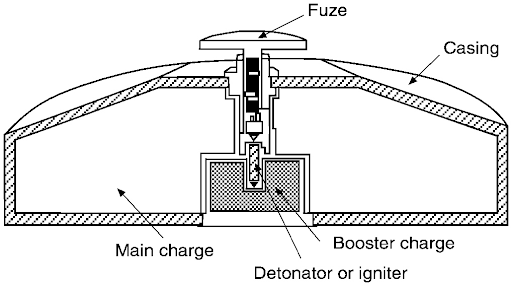
\includegraphics[width=\linewidth]{00 - Images/composition of vehicle landmine.png}
  \caption{Composition of Vehicle Landmine \cite{NAP10071}}
  \label{fig:composition of vehicle landmine}
\end{wrapfigure}

Landmines are explosive devices with an unmanned trigger mechanism. Landmines are constructed with the specific needs to either disable vehicles or personnel. The content of mines varies based on target area, but all mines have a trigger mechanism and a main explosive charge. Mines usually consist of an explosive chain reaction being initiated by the trigger mechanism. As in the case with figure xx2 the chronological order of initiation is the fuse then the detonator or ignited followed by the booster charge and finally the main charge. Landmines have different shapes and sizes based on their intended target. anti-personnel mines are usually small

\section{Explosions and pressure waves}

Explosive material is overall but into two types; low and high explosive. A low explosive material creates a pressure wave with enough force to push/move objects possibly at great velocity. High explosive material creates shockwaves that potentially crush objects at relatively close proximity (to the detonation) while pushing away anything in its radius. Low or high explosive refers to the burn rate of material. A pressure wave from an exploding landmine is usually created by expanding gasses released from the combustion of the main charge. This wave of pressurized gasses travels outwards from the explosion in all directions with its highest velocity in the beginning and then fast decelerates over the distance. At some point the wave moves backwards to fill out the vacuum created by the explosion at the origin point of the wave \cite{Siegelbook}.

\section{Landmines, their Placement and Trigger Mechanisms}

For an anti-personnel landmine to be effective against its subject  
For landmines to be effective against “enemy” forces they have to be hidden out of sight while close enough for its detonation to release a critical force upon the target/subject. Often range from 60-140 mm in diameter. \textbf{Anti-personnel} mines have two main ways of injuring the subjects;
\begin{enumerate}
    \item The force of the shock-wave crushing and “throwing” away the subject.
    \item The casing of the mine and its surrounding is accelerated in all directions by the explosion, penetrating objects in a large area
\end{enumerate}

\begin{wrapfigure}{R}{0.47\linewidth}
\centering
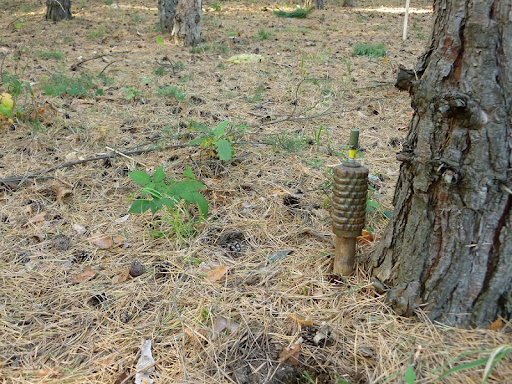
\includegraphics[width=\linewidth]{00 - Images/evolution-landmines-to-ieds.png}
  \caption{An AP Stake Mine with tripwire, Kosovo \cite{LinternWebsite}}
  \label{fig:An AP Stake Mine with tripwire, Kosovo}
\end{wrapfigure}
Mines meant to crush the victim with the pure force of the shock-wave has to be placed in close proximity to the target. One way to compensate for the distance is sizing up the explosive charge for a greater blast radius. The trigger mechanism for this type of mine is usually part of the casing of the mine, meaning the victim/target is required to disturb the mine directly. The most common trigger mechanism here is in integrated presurplate built into the mine requiring the victim/target to step on or possibly just close to it depending on the trigger’s sensitivity. The other type of anti-personnel landmines are \textbf{pre fragmented landmines} placed on or possibly over the ground with the main effect on victims being fragments of the outer casing and (as well as) the surrounding. The advantage here is a larger area of effect while the downside is the mine and the tripwire being visible as seen on figure \ref{fig:An AP Stake Mine with tripwire, Kosovo}. \textbf{Anti-vehicle} mines usually range from 1 - 20 kg and either target the wheels, control device and engine or the “belly” of the vehicle. 

%\section{One specific landmine:}
%The name, functionality and specifications/stats.

\section{Landmines in Warfare}

Deploying landmines in conventional warfare has been done in a wide variety of ways over the time. The most common is minefields laid by hand and usually mapped by combat engineers to make the removal of it more convenient. These landmines usually get hidden in the ground and they can be a combination of anti-personnel and anti-vehicle mines. It depends entirely on whether or not the armed forces have the capacity and the will to do so. In war it is not always possible to make an accurate map over the deployed mines location. Sometimes it comes down to the time required while other times it depends on the method of deployment e.g. with usage of cluster munition from artillery and aircrafts to deliver multiple mines at a time and even as an offencive do to the long range. With this method it is nearly impossible to make an accurate map of the newly deployed minefield as well as marking the minefield. Although they will be visible at first, they will end up blending in with nature over time and as years pass they may sink into the ground. In \textbf{conventional warfare} these fast but nearly impossible to map methods are often avoided because of their harmful effect on the land during and even after the war/conflict. A common use of landmines are minefields made with the purpose of leading the enemy forces into an disadvantageous position in the terrain, allowing friendly troops to take a favorable position turning it into a battlefield. This is all part of a defensive maneuver where the enemy has to choose between moving through the minefield or possible into an ambush. When preparing an ambush the defending army will choose an advantageous position, usually some sort of high ground. Then place or prepare an obstacle with the purpose of bringing the enemy to a full stop. When that happens the introding force would be taken under fire and forced to either push through the obstacle or fall back. Such obstacles could be large objects on the road blocking passage or barbed wire. It would likely be reinforced by numerous landmines to make the removal even more difficult and time consuming. At this point the attacking force would be desperate to breach through to the obstacle, possibly using explosives to speed up the process. Doing this mine from around the obstacle would be displaced and the entire maneuver would make it extremely difficult to find the landmines afterwards.

\section{Landmines in Conflict Zones}

For unconventional warfare there are no rules and thereby almost nothing to protect civilians as well as the land from being “affected” more than necessary by the conflict. In this chase it is unlikely that the unconventional force has access to mass production of landmines and therefore makes use of improvised solutions. This could involve re-purposing other types of munition into creative but unorthodox landmines and explosive devices also known as improvised explosive devices (IED).\\

\iffalse
\section*{All Sources in this Section}

Historical use of mines:\\ https://onlinelibrary-wiley-com.zorac.aub.aau.dk/doi/10.1002/9781444338232.wbeow414

\vspace{2mm}

Blast injuries:\\ https://tbi.cemmlibrary.org/Moderate-to-Severe-TBI/Mechanisms-of-TBI/Blast-Injuries 

\vspace{2mm}

Chemistry in explosions:\\ https://ebookcentral.proquest.com/lib/aalborguniv-ebooks/reader.action?docID=4182981&ppg=236 

\vspace{2mm}


Evolution landmines to IEDs:\\ https://neillintern.com/2017/12/15/evolution-landmines-to-ieds/ 

\vspace{2mm}

What is landmines:\\ https://www.nap.edu/read/10071/chapter/5#27 

\vspace{2mm}

Landmines and mine action:\\ http://web.mit.edu/demining/assignments/understanding-landmines.pdf 

\vspace{2mm}

Facts about landmines:\\ https://www.landminefree.org/2017/index.php/support/facts-about-landmines 

There has only been used sources from the above sources.
\fi


\iffalse
Mines are usually simple mechanisms that commonly consist of a container, the internal explosive material, and a trigger. These components can vary according to their intended purpose or accessibility \cite{LandmineDetectionTechniques2010}.


The container can be made with a variety of different materials, ex. plastic, wood, metal, or a combination of those three \cite{LandmineDetectionTechniques2010}. This raises a problem for the mine detection techniques since the materials and size of the explosive device can vary a lot. Improvised mines are usually made with materials available at hand \cite{DetectionAndLocalizationOfImprovisedDevices2010}. That includes both the casing, the explosive material, and the trigger. The trigger component is what will detonate the mine. The mine could be activated by an electronic or pressure sensor. If the mine is intended as an anti-personnel mine with a pressure sensor, then it usually requires a pressure between 5-16 kg to initiate. Anti-tank mines require more than 100kg pressure to initiate. Some mines are buried just below the ground while others have their triggers above the ground \cite{LandmineDetectionTechniques2010}.


The most common purpose of landmines and unexploded ordnance (UXO) is not necessarily to kill the victim, but to disable personnel and/or equipment. This can result in long-term medical and psychological trauma, as well as being a financial burden for the affected individuals. As well as the mine action, see Figure \ref{fig:contributions_by_thematic_sector_2018}. Areas covered in mines can restrict access to clean water, arable land, roads, healthcare services, and facilities \cite{OxfordAcademic2005}. Therefore, it is easy to see the benefits that can be gained from demining. 
\fi
\chapter{Current market}

The process of humanitarian demining consists mainly of three aspects, firstly to prepare the terrain or mine-affected area. This includes removing objects and clearing of vegetation, which is mostly done by heavily armoured vehicles. That process usually triggers some of the mines but not all. Secondly is to precisely locate the mine and thirdly to remove or destroy it \cite{HiddenKillers2019}.

New technology should try to help in one of these areas. Multiple methods for demining have been developed since the introduction of landmines in warfare. These methods vary from, training and using animals for mine localisation, to using advanced technology for localisation and demining. Regarding this, advanced technologies are in use, these are however mostly reserved for the military \cite{HiddenKillers2019}.
The process of military demining is in some ways like humanitarian demining. However, it is different in the way, that the goal is not to clear the minefields and make them safe for civilian use, but to make a safe passage through the minefields \cite{HiddenKillers2019}. A comparison between these, military and humanitarian demining, can be seen in Figure \ref{fig:military_humanitarian_demining}.

\medskip

\begin{figure}[h]
  \centering
      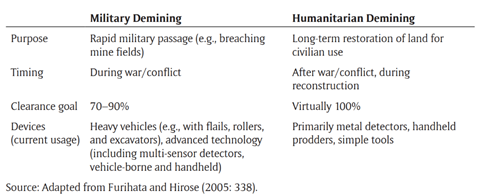
\includegraphics[width=1\textwidth]{00 - Images/military_humanitarian_demining.png}
  \caption{Comparison of Military and Humanitarian Demining \cite{HiddenKillers2019}}
  \label{fig:military_humanitarian_demining}
\end{figure}

In military demining-operations, armoured machines or vehicles are often used since they activate the mines and hereby destroy them. Nevertheless, these vehicles have shown to be ineffective in difficult terrain and are mostly reserved for the military \cite{6LeggedRobot2007}. Even though advancements in technology are being made, they still need more development, testing, and a cost reduction, before they can be properly implemented by humanitarian workers \cite{HiddenKillers2019}. 

\section{Manual demining methods}

\subsection{metal detectors}

a metal detector i used to measures disturbances in magnetic fields caused by metal objects in the ground. the problem with this is that it is a very slow process.

\subsection{mine prodding}
Mine prodding Which is accomplished by using some form of prodding tool a trowel, bayonet or something of similar length and sharpness. When mine prodding the goal is to ascertain the location of a mine that has previously been located by a metal detector. The prod is inserted in the dirt at around a 30 degree angle and it is then pushed into the ground with the goal of hitting the mine at an angel so as to avoid the triggering mechanism. Mine prodding is only used in the excavating of mines that have been found using a metal detector or similar method in humanitarian demining as it is considered to be to dangerous to use for locating mines.

\subsection{animals in demining}
Attempts to use animals to locate mines have proven somewhat use full; A example of this dogs and rats have been used for locating mines. Dogs have proven somewhat use full in this regard as they can be trained to sniff out the explosives. The problem with using dogs for locating mines is that the dogs get often get confused if there is more than one source of the smell they are trying to locate \cite{DeminingDogs2016}. Rats can be trained for this as well but have not had this problem\cite{PouchedRats2016}. Another problem in the use of animals is that you can not be as methodical in your search as you might like.

\subsection{visual inspection}
Locating a mine using visual detection. Is as the name implies to attempt to locate mines using vision. While the accuracy of a visual inspection can be improved with knowledge of mines and methods of hiding them it is still not a very trustworthy method for locating\cite{LandmineDetection2000}.

\begin{figure} [H]
    \centering
    \begin{subfigure}[b]{0.28\textwidth}
        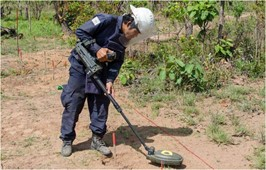
\includegraphics[width=\textwidth]{00 - Images/man_with_detector.jpg}
        \caption{Finding landmines with metal detector \cite{ManDetector2018}}
        \label{fig:man_with_detector}
    \end{subfigure}
    ~ %add desired spacing between images, e. g. ~, \quad, \qquad, \hfill etc. 
      %(or a blank line to force the subfigure onto a new line)
    \begin{subfigure}[b]{0.28\textwidth}
        
\includegraphics[width=\textwidth]{00 - Images/rat_finding_mines.jpg}
        \caption{Rats sniffing out bombs}
        \label{fig:rat_finding_mines}
    \end{subfigure}
    ~ %add desired spacing between images, e. g. ~, \quad, \qquad, \hfill etc. 
    %(or a blank line to force the subfigure onto a new line)
    \begin{subfigure}[b]{0.28\textwidth}
        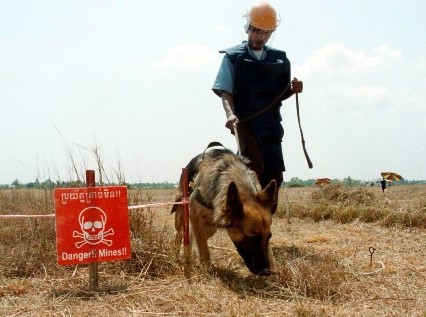
\includegraphics[width=\textwidth]{00 - Images/dog_finding_mines.jpg}
        \caption{Dogs sniffing out landmines}
        \label{fig:dog_finding_mines}
    \end{subfigure}
    %\caption{Pictures of animals}\label{fig:animals}
\end{figure}

It becomes very clear that advancements and innovations in humanitarian demining should be made. Robots could be a huge help in demining an area since they potentially eliminate the human risk associated with detecting landmines. Multiple demining robots have already been made with the intent of finding and/or disposing landmines and unexploded ordinance. These robots each work very differently and use different technology to detect landmines all to make the demining process easier, faster, and safer \cite{MotionPlanningRobot2011}.

\section{Current Demining Robots}

In general, modern humanitarian ground-based demining robots can be divided into three categories, based on movement types.
\begin{itemize}
\setlength{\itemsep}{0.05\baselineskip}
	\item Continuous track robots
	\item Wheeled robots
	\item Legged robots
\end{itemize}

Each of these types has its strengths and weaknesses. Where continuous tracked and wheeled robots provide easy accessibility, since most of the parts required for construction can be found in local existing technologies, their contact to the ground is high, which increases the risk of accidentally triggering a mine. Opposite to this, the legged robots have a smaller contact area with the ground and therefore run with a smaller risk of triggering. On top of this, legged robots provide omnidirectional movement, i.e. it can change directions while not needing to make a turn, ex. going in one direction, stopping, continue in 27 degrees left from the previous direction. This derivatively decreases the risk of accidental triggers even more \cite{6LeggedRobot2007}. However, we assume these robots require more advanced mechanical systems, which increases cost, and the need for specialised parts that are less likely to be found in the local area where the demining takes place. Wheels can be made omnidirectional as well, but that solution is not suitable for rough terrain, due to various places that dirt can get stuck.\\

It is our opinion that the tracked and wheeled solutions outweigh the legged robots in the current market, mainly for their simplicity in both construction, system, and operator requirements. Furthermore, we assume that wheels are cheaper than tracks, due to fewer parts, needed to construct a wheel, than a track. Therefore, we want to work with a wheeled robot.\\

Humanitarian demining robots can likewise be divided into 3 categories based on autonomy, as such:
\begin{itemize}
\setlength{\itemsep}{0.05\baselineskip}
	\item Fully operator-controlled robots
	\item Semi-autonomous robots
	\item Fully autonomous robots
\end{itemize}

A fully operator-controlled robot can have a simple design. But these robots require a highly qualified/trained operator, to make full use of the robot. We assume that these operators are hard to come by in the local area, this can be thought of as an issue for these types of robots.\\

Moving up the categories to more autonomous solutions, would, of course, be a more ideal solution because this would decrease human error and the human risk factor, i.e. operator will not be close to a possible explosion. However, this, as with anything else, comes with higher expenses and without further improvements on the robots, to lower the expenses it could be difficult to make them it more affordable \cite{6LeggedRobot2007}. Although we assess that a fully autonomous solution will be cheaper in the long run, based on operating expenses. Therefore, we prefer a fully autonomous solution.

\section{Sensors}

We already provided information on less advanced methods for mine detection, see ‘Primitive demining methods’, however more advanced technology such as the use of detection sensors could provide a safer alternative. These sensors can be divided into the following groups \cite{HumanitarianDemining2017}:
\begin{itemize}
\setlength{\itemsep}{0.05\baselineskip}
	\item Explosive detectors
	\item Electromagnetic sensors
	\item Electro-optic sensors
\end{itemize}

Explosive detectors are used to detect the explosive material of a mine. Electromagnetic sensors, such as metal detectors (MD), which are used to measure magnetized metals, or ground penetrating radar (GPR), which can identify plastic. An electro-optic sensor such as an infrared sensor (IR), uses light waves to measure the distance to some objects in the soil. All these could potentially be used to locate mines \cite{HumanitarianDemining2017}.

Limitations on these sensors do exist, which is why a combination of multiple sensors might be the best option for a mine detection robot. For instance, an electro-optic sensor such as an infrared sensor cannot be used to centre specific mines. This means they are only capable of scanning an area. Ground-penetrating radar is relying on the ground condition to determine the depth of its ground penetration but can however detect other materials than metal beneath the ground. Metal detectors might be cheap and reliable but can, as the name implies, only detect metal \cite{HumanitarianDemining2017}.
So in general, making a robot effective, means using a few different sensors and detectors to cover the limitations of the single one \cite{6LeggedRobot2007}.

\section{Current Humanitarian Demining Robots}

Since humanitarian demining still heavily relies on dangerous primitive techniques, a lot of re-search is being done with the intent of creating a viable robot to be used in humanitarian demining. Figure \ref{fig:field_robots_for_humanitarian_demining_2014} shows a table, which is taken from \cite{FieldRobots2014}. It presents six modern-day field robots with different specifications, all of which have been presented as a possible solution to the demining problem \cite{FieldRobots2014}.
\begin{figure}[h]
  \centering
      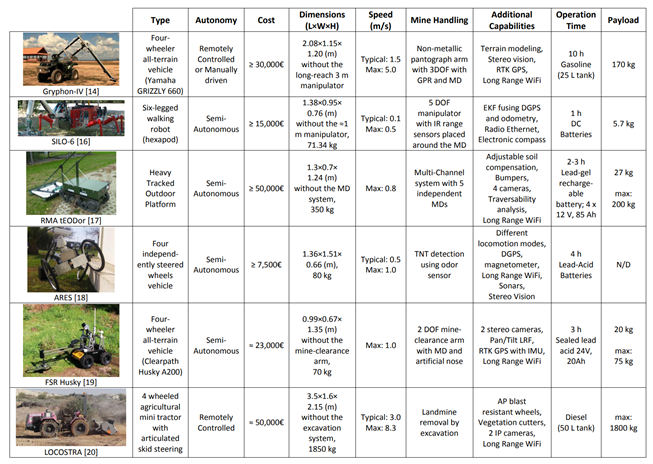
\includegraphics[width=1\textwidth]{00 - Images/field_robots_for_humanitarian_demining_2014.png}
  \caption{Deploying field robots for humanitarian demining: Challenges, requirements, and research trends, 2014 \cite{FieldRobots2014}}
  \label{fig:field_robots_for_humanitarian_demining_2014}
\end{figure}

As seen in Figure \ref{fig:field_robots_for_humanitarian_demining_2014} these demining robots vary a lot in terms of design, cost, size, sensor technology, and operation time. Some are made with the intent of removing mines and some only to locate them \cite{FieldRobots2014}. We will only specify robots used for detecting mines. The robots have different qualities which makes them relevant in the specific context they were built to handle. For example, the ARES robot in Figure \ref{fig:field_robots_for_humanitarian_demining_2014} might be relatively lightweight (80 kg) and cheap ($\ge$ 7.500€) but are only capable of detecting the explosive TNT.\\

Following this is a presentation of some current demining robots. These are chosen to give insight into the various pros and cons, that the current day robots have to offer. The presentation will include some of the major aspects of the robots, and the usefulness that they each provide. In addition, the mentioned robots will illustrate the diversity in demining robots and how some of their specifications give an advantage or disadvantage when detecting mines.

\subsection{CSIRO, Data61, and Molten Labs}

\begin{wrapfigure}{r}{0.5\textwidth}
    \centering
      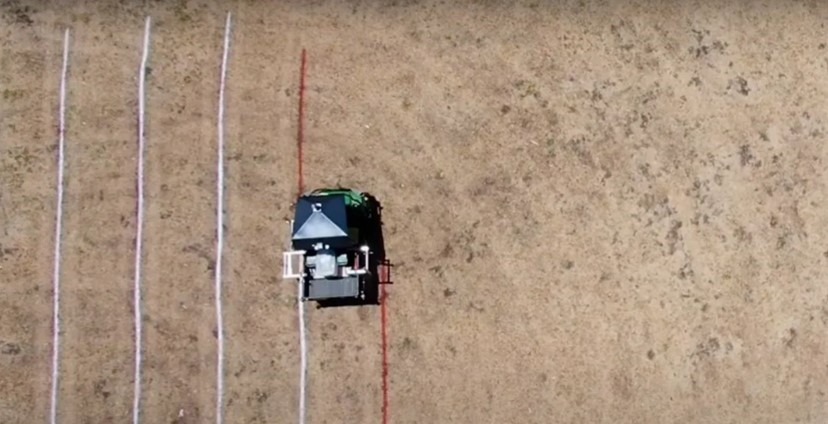
\includegraphics[width=0.45\textwidth]{00 - Images/autonomous_ground_vehicle_for_landmine_clearance.jpg}
  \caption{Autonomous Ground Vehicle for Landmine Clearance \cite{CSIRO2020}}
  \label{fig:autonomous_ground_vehicle_for_landmine_clearance}
\end{wrapfigure}
This is a newly developed mine detection and clearing robot, which uses metal detector sensors to detect mines and could be fitted with a powerful torch that can incinerate mines. We selected this robot because of its ability to collaborate between multiple robots of the same type and the ability to visualize cleared areas. The robot, which is said to approximately be the size of a golf cart, is developed by CSIRO, Data61, and Molten Labs. The robot is fully autonomous and is intended to work together with multiple robots of the same kind. These robots can attach to each other, which also makes them able to drag a malfunctioned robot out of the contaminated area. Furthermore, it allows for quicker mine-clearing when multiple robots are working together. This robot uses a spray-painting system to physically mark the ground that visually shows the areas which have been cleared of mines \cite{CSIRO2020}. It however is a big machine and it could be a troublesome endeavour to deploy multiple robots in a remote area.


\subsection{HUMI}

\begin{wrapfigure}{r}{0.5\textwidth}
    \centering
      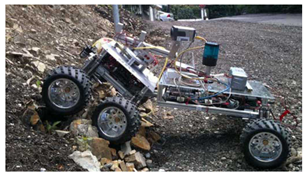
\includegraphics[width=0.45\textwidth]{00 - Images/humi_a_mobile_robot_for_landmine_detection.png}
  \caption{HUMI; A Mobile robot for landmine detection \cite{HUMI2012}}
  \label{fig:humi_a_mobile_robot_for_landmine_detection}
\end{wrapfigure}
This is a six-wheeled semi-autonomous robot used for detecting landmines. We have chosen this robot because of its weight and size. Even though this robot is only a prototype, a demining robot which is based on the prototype HUMI, has been set into full-scale production. HUMI is a light-weight (24,4 kg) demining robot made to be cost-effective. This means that the robot uses cheap available technology such as a landmine detector and its controller. The robot relies heavily on being small, cheap, and easy to use. Its shortcomings are that it is not fully autonomous, only relies on a single metal detector, and that the perception sensors were not available at a reasonable price when it was made \cite{HUMI2012}.

\subsection{ClearPath Husky}

\begin{wrapfigure}{r}{0.5\textwidth}
    \centering
      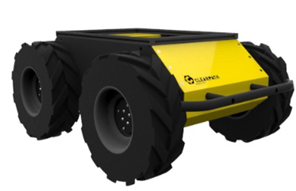
\includegraphics[width=0.45\textwidth]{00 - Images/husky_unmanned_ground_vehicle_robot.png}
  \caption{Husky: Unmanned Ground Vehicle-Robot \cite{ClearPath2020}}
  \label{fig:husky_unmanned_ground_vehicle_robot}
\end{wrapfigure}
This robot is a four-wheeled all-terrain robot. We included this one because of the modularity it provides. This is the main advantage of it. While not specifically designed for demining, ClearPath offers a broad variety of packages to the robot, which can allow the robot to do a multiple of different tasks. The manipulator package is the most ideal package for a demining purpose, this pack-age includes a robotic arm. Of course, this should be in a combination with a metal detector and/or other types of detectors \cite{ClearPath2020}. This was done in the HRATC 2015 competition, which is a community demining competition, in which the goal is to create the best search and mapping algorithm \cite{HRATC2015}. The Husky provides a great traverse ability and can carry a high payload, even in rough terrains. The Husky is priced somewhere in the middle of the price range, as seen in Figure 8. However, it lacks a purposefully designed software for a humanitarian demining operation \cite{ClearPath2020}.\\

An example of the types of sensor which could be used can be seen in Figure \ref{fig:field_robots_for_humanitarian_demining_2014}.

\subsection{SILO-6}

\begin{wrapfigure}{r}{0.5\textwidth}
    \centering
      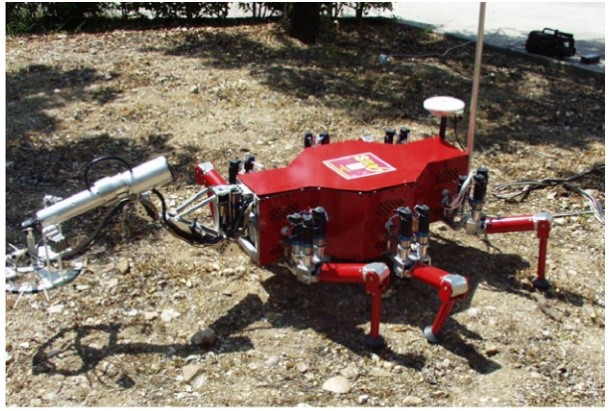
\includegraphics[width=0.45\textwidth]{00 - Images/silo_6_in_action.jpg}
  \caption{SILO-6 In action \cite{6LeggedRobot2007}}
  \label{fig:silo_6_in_action}
\end{wrapfigure}
This robot is also mentioned in Figure \ref{fig:field_robots_for_humanitarian_demining_2014}. It provides a very interesting design, which is very different from the rest of the spectrum. We have selected this because of the six-legged platform which is different from the other examples. This makes it very mobile even in rough terrain and gives a lot of freedom when moving because of the independently moving legs. Six legs have proven to increase stability compared to four legs and are stable in natural terrain which is important when using some sensing technologies. It is fitted with a metal detector but could be getting additional sensors if needed. It is a relatively lightweight (71,34 kg) semi-autonomous robot \cite{6LeggedRobot2007}. This robot could however be hard to replace or do repair work on. Its legs most likely require specially made parts.  

\section{Issues with Current Solutions}

The current solutions have a lot of potential in helping humanitarian demining. Although there is a reason why they are not already hugely implemented in humanitarian work. Every robot has its compromises. It is our intent, to identify and summarise these compromises.

Some of the major issues of the current use of robots, involve oversized robots. Most of them weigh over 70 kg. This increases the chance of accidentally activating a mine. HUMI is the only light robot, but this also limits the available space for sensors. But with optimization, and newer technologies available, it should be possible to fit other sensors as well. Robots that weigh hundreds of kilograms and are based on all-terrain vehicles (ATV) or golf carts provide issues regarding transportation. Other robots are limited in the lack of software, and some are limited because of the potential price to repair parts. Most solutions are quite expensive as shown in Figure \ref{fig:field_robots_for_humanitarian_demining_2014} and this cost would properly be an issue for many humanitarian organizations’ budgets. Overall, most of the robots are good solutions, but we propose a solution which also takes these aspects into consideration.
\chapter{Statements}

\section{Final Problem Statement}

With the regard to current \gls{sota} demining robots, how to, with a new demining robot product, make improvements on the \gls{sota} areas regarding the speed and proficiency in locating, and mapping, mines in heavily contaminated areas in Afghanistan.

\section{Delimitation}

Due to time constrain, designing a new demining robot product that could satisfy the needed requirements in the final statement, i.e. increased speed in localisation and mapping, maneuverability on any surface other than on an indoor flat surface, we made a delimited problem statement.

\section{A Delimited Problem Statement}\label{delimit_statement}

How we get the Turtlebot 2e to act as proof of concept for the part of our final problem statement which addresses the need for an algorithm to make a robot map an area while in the process of locating objects which have the same attributes as various landmines    
% https://www.productplan.com/glossary/moscow-prioritization/

\chapter{Requirements}

% Indtroduktion til kravsspecifikation
Detection robots should be developed to assist in demining in the best possible way, and it is advisable to specify the system and the mechanics of the robot to produce a testable prototype. With this in mind, the project group has derived requirements for the mobile-robot. The requirement specifications are based on the knowledge gained in the problem analysis. These sections imply what detection robots should be able to do, as well as the legislation which must be followed during the design of the robot. These requirements must be met for the robot to effectively work as a detection robot. Likewise, our must- and should-have requirements have been founded on our knowledge of existing robots and literature\\

        \vspace{2mm}

The following requirements are set by the MoSCoW method for requirements specification followed by a suitable test method for the given requirement.

\begin{itemize}[label={}]
\setlength{\itemsep}{0.05\baselineskip}
    \item \framebox[\mylen][c]{\large{\textbf{M}}} \normalsize Must Have: \hspace{5mm} Non-negotiable requirements that is mandatory for the project group \par
    \item \framebox[\mylen][c]{\large{\textbf{S}}} \normalsize Should Have: \hspace{1.8mm} Important requirements that are not vital, but add significant value \par
    \item \framebox[\mylen][c]{\large{\textbf{C}}} \normalsize Could Have: \hspace{3.5mm} Nice to have requirements that will have a small impact if left out \par
    \item \framebox[\mylen][c]{\Large{\textbf{W}}} \normalsize Will Not Have: Requirements that are not a priority for this specific time frame \par
\end{itemize}

\vspace{4mm}

\iffalse
\begin{enumerate}
    \item Move from A-B 
    
    \vspace{-6mm}
    
    \item Moving in terrain
    
    \vspace{-6mm}
    
    \item SLAM (Simultaneous Localization And Mapping)
    
    \vspace{-6mm}
    
    \item Avoid triggering landmines, driving off a cliff or hitting objects
    
    \vspace{-6mm}
    
    \item Search for metal
    
    \vspace{-6mm}

    \item Enough power for hardware (battery/power source)
    
    \vspace{-6mm}    
    
    \item Reusable (battery/fuel)
    
    \vspace{-6mm}
    
    \item Can be refueled and or recharged
    
    \vspace{-6mm}
    
    \item Mark landmines location in a physical world
    
    \vspace{-6mm}
    
    \item Mark landmines location in a virtual map
    
    \vspace{-6mm}
    
    \item Resistant to environment
    
    \vspace{-6mm}
    
    \item Battery time
    
    \vspace{-6mm}
    
    \item Battery time
    
    \vspace{-6mm}
    
    \item Moveable sensors
    
\end{enumerate}
\fi

\newpage

\section{Must Have}

\subsection{Move from A-B}\label{R1}
The robot should be able to move from A to B.

\subsubsection*{Testing Strategy}
This will be tested by having the robot move from one point to another.

%%%%%%

\subsection{Moving in Terrain}\label{R2}
More than just moving, it should be able to do so in difficult terrain; move up and down hills, over soft ground, through tall grass and smaller branches.

\subsubsection*{Testing Strategy}
This will be tested by having the robot move around in various terrain. the terrain it will be tested in will be as follows. loose sand, mountain areas. lightly vegetated terrain and tall grass.

%%%%%%

\subsection{SLAM (Simultaneous Localization And Mapping)}\label{R3}
Find its own location, map its movement, make a route that covers the entire area while avoiding obstacles by adapting the route.

\subsubsection*{Testing Strategy}
Place the robot within an area and let it “search”, then see if it gets stuck or leaves out areas. if it does then it is a fail.

%%%%%%

\subsection{Avoid triggering landmines, driving off a cliff or hitting objects}\label{R4}
Use sensor data to locate obstacles such as trees, stones, cliffs and other non-passable areas along the route as well as tripwire.

\subsubsection*{Testing Strategy}
Set up different obstacles with the search area and let it search the area, if it collides with any of them then it is a fail.

%%%%%%

\subsection{Search for metal}\label{R5}\todo[]{find bedre formulering - Ikke nødvendig at det skal være metal detektor fordi at den praktiske robots bare representerer input.}
Search the area in and above for metal. 

\subsubsection*{Testing Strategy}
Place metal below and above the ground and see if it can find it. if it does not find all then it is a fail.

%%%%%%
 
\subsection{Enough power for hardware (battery/power source)}\label{R6}
Have a power source.

\subsubsection*{Testing Strategy}
See if it can turn on and use all functions if not then it is a fail.

%%%%%%

\subsection{Reusable (battery/fuel)}\label{R7}
Can be refueled and or recharged.

\subsubsection*{Testing Strategy}
Refill/recharge the machine with the chosen source of power.

%%%%%%

\subsection{Can be refueled and or recharged}\label{R8}
Have a power source.

\subsubsection*{Testing Strategy}
Refill/recharge the machine with the chosen source of power.

%%%%%%

\subsection{Mark landmines location in a physical world}\label{R9}
Be able to mark locations of the objects it is searching for in a physical world.

\subsubsection*{Testing Strategy}
Have the machine locate and object in its intended terrain and use the chosen marking method on the object's location.

%%%%%%

\subsection{Mark landmines in a virtual map}\label{R10}
Be able to mark locations of the objects it is searching for in a virtual map.

\subsubsection*{Testing Strategy}
Have the machine locate and object in its intended terrain and use the chosen marking method in the virtual map.


%%%%%%

\newpage

\subsection{Resistant to environment}\label{R11}
It must be able to function in the Afghan climate. This is to say, be able to handle the local temperatures and other natural hazards such as sand and rain.

\subsubsection*{Testing Strategy}
Can be tested by having it run in temperatures that range from the chosen location’s minimum temperature to its maximum temperature. preferably at both lower and higher temperatures than necessary. have it run while sand is being poured on it and have it run while water is being poured on it.


%%%%%%%%%%%%%%%%%%%%%
% SHOULD HAVE SECTION

\section{Should Have}

\subsection{Battery time}\label{R12}
The robot should have a power source that enables it to operate it's intended tasks for XX hours.

\subsubsection*{Testing Strategy}
Calculation of the robots battery time followed by a series of runtime tests to conclude the calculations

%%%%%%%%%%%%%%%%%%%%
% COULD HAVE SECTION

\section{Could Have}

\subsection{Moveable sensors}\label{R13}
The robot can move the sensors to more precisely pinpoint landmine locations in the ground

\subsubsection*{Testing Strategy}

\section{Will Not Have}

This section will be taken into use in the practical requirements (chapter \ref{prac_req})


\newpage


\section{Safety of Machinery}
When designing a robot, standardization/legislation can not be disregarded as a focus point, thus the robot should be designed in correlation to the following standards for security measures and international (ISO) standardisation of robotics.

\vspace{2mm}

To accommodate the Machine Directive 2006/42/EC, which is required for the robot to be CE marked, the robots should be designed with the following standards in mind

\begin{itemize}
\setlength{\itemsep}{0.05\baselineskip}
\item \textbf{Emergency stop}\\
The robot should have an emergency stop as a security measure, if unintended behaviour appears in correlation to DS/EN ISO 13850:2015

\item \textbf{Safety-related parts of control systems}
\begin{itemize}
\setlength{\itemsep}{0.05\baselineskip}
\item Principles of design DS/EN ISO 13849-1:2015
\item Validation DS/EN ISO 13849-2:2014
\end{itemize}

\item \textbf{Requirements for wireless control systems of machinery}\\
The robot are to be designed in correlation with DS/EN 62745:2017, which describes communication between portable operator control stations and the robot

\item \textbf{Degrees of protection provided by enclosures}\\
The robot should be designed with a rating of IP-64
In correlation to DS/EN 60529+A1:2002

\item \textbf{Coordinate and motion nomenclatures}\\
Movement in an coordinate system based map should be standardized\\
in correlation to DS/ISO 9787

\item \textbf{Collaborative robots (Collision detection)}\\
The robot should be tested in regard to the limiting values of collision detection described in DS/ISO/TS 15066

\item \textbf{Risk assessment}\\
A risk assessment should be performed to ensure a decrease of potential security risks in regards to DS/EN ISO 12100:2011
\end{itemize}

\newpage

\chapter{Practical requirements}\label{prac_req}

Within the time frame of this project the project group plan to have the Turtlebot 2e act as proof of concept as stated in the delimited problem statement (Section \ref{delimit_statement}), thus all of the requirements are not able to be met and must be delimited in regard for the problem statement. Therefore a list of practical requirements is listed in the following section, which takes this into account. Test methods will be as stated in the requirements chapter.

\vspace{-3mm}

%%%%%%%%%%%%%%%%%%%%%%%
% MUST HAVE SECTION
\vspace{-1mm}

\section*{Must Have}
\begin{itemize}

    \vspace{-3.5mm}

\item Moving (section \ref{R1})

    \vspace{-3.5mm}

\item SLAM (Simultaneous Localization And Mapping) (section \ref{R3})

    \vspace{-3.5mm}

\item Avoid triggering landmines, driving off a cliff or hitting objects (section \ref{R4})

    \vspace{-3.5mm}

\item Search for metal  (section \ref{R5})

    \vspace{-3.5mm}

\item Enough power for hardware (battery/power source)  (section \ref{R6})

    \vspace{-3.5mm}

\item Reusable (battery/fuel)  (section \ref{R7})

    \vspace{-3.5mm}

\item Can be refueled and or recharged  (section \ref{R8})

    \vspace{-3.5mm}

\item Mark landmines location in a physical world  (section \ref{R9})

    \vspace{-3.5mm}

\item Mark landmines location in a virtual map  (section \ref{R10})
\end{itemize}

%%%%%%%%%%%%%%%%%%%%%%%
% SHOULD HAVE SECTION
\vspace{-2mm}

\section*{Should Have}
\begin{itemize}

    \vspace{-3.5mm}

\item Battery time  (section \ref{R12})

\end{itemize}

%%%%%%%%%%%%%%%%%%%%
% COULD HAVE SECTION
\vspace{-2mm}

\section*{Could Have}

    \vspace{-3.5mm}
    
Not significant for this requirement section

%%%%%%%%%%%%%%%%%%%%%%%
% WILL NOT HAVE SECTION
\vspace{-2mm}

\section*{Will Not Have}
\begin{itemize}

    \vspace{-3.5mm}

\item Moving in terrain (section \ref{R2})

    \vspace{-3.5mm}

\item Resistant to environment  (section \ref{R11})

    \vspace{-3.5mm}

\item Moveable sensors (section \ref{R13})
\end{itemize}





     
    
    
     
    
     
    
     
    
     
    
     
    
     
    
     
    
     
    
     
    
     
    
    
     








\newgeometry{left=0.2cm,right=0.2cm}
\begin{center}
\begin{longtable}{| c | L{4cm} | L{6cm} | L{4cm} |}
\caption{Requirements} \label{tab:long} \\
\hline \multicolumn{1}{|c|}{\textbf{\#}} & \multicolumn{1}{c|}{\textbf{Name}} & \multicolumn{1}{c|}{\textbf{Description}} & \multicolumn{1}{c|}{\textbf{Testing section}}\\ \hline 
\endfirsthead

\multicolumn{3}{c}%
{{\bfseries \tablename\ \thetable{} -- continued from previous page}} \\
\hline \multicolumn{1}{|c|}{\textbf{\#}} & \multicolumn{1}{c|}{\textbf{Second column}} & \multicolumn{1}{c|}{\textbf{Third column}} & \multicolumn{1}{c|}{\textbf{Fourth column}}\\ \hline 
\endhead

\hline \multicolumn{4}{|r|}{{Continued on next page}} \\ \hline
\endfoot

\hline \hline
\endlastfoot

1\label{req8.1} & Mapping & The robot should be able to map the surrounding environment to a .pgm image file with corresponding .yaml definition file & Section(x.x) \\
\hline
3 & Map Structure & The robot should be able to divide a given environment map into a grid with a width of 350mm, for the purpose of plotting a search route & Section(x.x)\\
\hline
2 & Navigation & The robot should be able to navigate autonomously through a variety of terrains in Afghanistan, using the .yaml environment map & Section(x.x) \\ 
\hline 
4 & Obstacle avoidance & The robot should be able to detect obstacles in its current path, thus interrupt the current path and calculate a new path, furthermore the robot should avoid previous located mines \label{req.4} & Section(x.x) \\
\hline
5 & Mine detection & The robot should be able to detect mines made of metal and/or other materials such as plastic or glass, furthermore it should be able to approximate which type of mine it has located. & Section(x.x) \\
\hline
6 & Mine triggering & The robot should not exceed a weight of $\sim$6kg to ensure that it does not trigger landmines when approximating these. & Section(x.x) \\
\hline
7 & Runtime & The robot should have $\sim$8 hours runtime, furthermore the robot should be able to plan a route to the charging station autonomously (with respect to table \ref{req8.1} - \#4), to supplement a lower capacity battery & Section(x.x) \\
\hline
8 & abcdef ghjijklmn & 123.456778 & 8888 \\
9 & abcdef ghjijklmn & 123.456778 & 8888 \\
10 & abcdef ghjijklmn & 123.456778 & 8888 \\
11 & abcdef ghjijklmn & 123.456778 & 8888 \\
12 & abcdef ghjijklmn & 123.456778 & 8888 \\
13 & abcdef ghjijklmn & 123.456778 & 8888 \\
14 & abcdef ghjijklmn & 123.456778 & 8888 \\
15 & abcdef ghjijklmn & 123.456778 & 8888 \\
16 & abcdef ghjijklmn & 123.456778 & 8888 \\
17 & abcdef ghjijklmn & 123.456778 & 8888 \\
18 & abcdef ghjijklmn & 123.456778 & 8888 \\
19 & abcdef ghjijklmn & 123.456778 & 8888 \\
20 & abcdef ghjijklmn & 123.456778 & 8888 \\
T & abcdef ghjijklmn & 123.456778 & 8888 \\
One & abcdef ghjijklmn & 123.456778 & 8888 \\
One & abcdef ghjijklmn & 123.456778 & 8888 \\
One & abcdef ghjijklmn & 123.456778 & 8888 \\
One & abcdef ghjijklmn & 123.456778 & 8888 \\
One & abcdef ghjijklmn & 123.456778 & 8888 \\
One & abcdef ghjijklmn & 123.456778 & 8888 \\
One & abcdef ghjijklmn & 123.456778 & 8888 \\
One & abcdef ghjijklmn & 123.456778 & 8888 \\
One & abcdef ghjijklmn & 123.456778 & 8888 \\
One & abcdef ghjijklmn & 123.456778 & 8888 \\
One & abcdef ghjijklmn & 123.456778 & 8888 \\
One & abcdef ghjijklmn & 123.456778 & 8888 \\
One & abcdef ghjijklmn & 123.456778 & 8888 \\
One & abcdef ghjijklmn & 123.456778 & 8888 \\
One & abcdef ghjijklmn & 123.456778 & 8888 \\
One & abcdef ghjijklmn & 123.456778 & 8888 \\
One & abcdef ghjijklmn & 123.456778 & 8888 \\
One & abcdef ghjijklmn & 123.456778 & 8888 \\
One & abcdef ghjijklmn & 123.456778 & 8888 \\
One & abcdef ghjijklmn & 123.456778 & 8888 \\
One & abcdef ghjijklmn & 123.456778 & 8888 \\
One & abcdef ghjijklmn & 123.456778 & 8888 \\
One & abcdef ghjijklmn & 123.456778 & 8888 \\
One & abcdef ghjijklmn & 123.456778 & 8888 \\
One & abcdef ghjijklmn & 123.456778 & 8888 \\
One & abcdef ghjijklmn & 123.456778 & 8888 \\
One & abcdef ghjijklmn & 123.456778 & 8888 \\
One & abcdef ghjijklmn & 123.456778 & 8888 \\
One & abcdef ghjijklmn & 123.456778 & 8888 \\
One & abcdef ghjijklmn & 123.456778 & 8888 \\
One & abcdef ghjijklmn & 123.456778 & 8888 \\
One & abcdef ghjijklmn & 123.456778 & 8888 \\
One & abcdef ghjijklmn & 123.456778 & 8888 \\
One & abcdef ghjijklmn & 123.456778 & 8888 \\
One & abcdef ghjijklmn & 123.456778 & 8888 \\
One & abcdef ghjijklmn & 123.456778 & 8888 \\
One & abcdef ghjijklmn & 123.456778 & 8888 \\
One & abcdef ghjijklmn & 123.456778 & 8888 \\
One & abcdef ghjijklmn & 123.456778 & 8888 \\
One & abcdef ghjijklmn & 123.456778 & 8888 \\
One & abcdef ghjijklmn & 123.456778 & 8888 \\
One & abcdef ghjijklmn & 123.456778 & 8888 \\
One & abcdef ghjijklmn & 123.456778 & 8888 \\
One & abcdef ghjijklmn & 123.456778 & 8888 \\
One & abcdef ghjijklmn & 123.456778 & 8888 \\
One & abcdef ghjijklmn & 123.456778 & 8888 \\
One & abcdef ghjijklmn & 123.456778 & 8888 \\
One & abcdef ghjijklmn & 123.456778 & 8888 \\
One & abcdef ghjijklmn & 123.456778 & 8888 \\
One & abcdef ghjijklmn & 123.456778 & 8888 \\
One & abcdef ghjijklmn & 123.456778 & 8888 \\
One & abcdef ghjijklmn & 123.456778 & 8888 \\
One & abcdef ghjijklmn & 123.456778 & 8888 \\
One & abcdef ghjijklmn & 123.456778 & 8888 \\
One & abcdef ghjijklmn & 123.456778 & 8888 \\
One & abcdef ghjijklmn & 123.456778 & 8888 \\
One & abcdef ghjijklmn & 123.456778 & 8888 \\
One & abcdef ghjijklmn & 123.456778 & 8888 \\
One & abcdef ghjijklmn & 123.456778 & 8888 \\
\end{longtable}
\end{center}
\restoregeometry

%\chapter{Description}


%\chapter{Delimitations}


%\chapter{Conclusion}


\chapter{code}

\section{make\_box}

\begin{lstlisting}

#include <cstdlib>
#include <ros/ros.h>
#include <geometry_msgs/Twist.h>
#include <turtlesim/TeleportAbsolute.h>
#include <turtlesim/SetPen.h>

int main(int argc, char *argv[]) {
  ros::init(argc, argv, "make_box");

  float box_size = ros::param::param("~box_size", 9.0);

  ros::NodeHandle nh;

  ros::service::waitForService("/turtle1/teleport_absolute", -1);

  ros::ServiceClient teleport_client = nh.serviceClient<turtlesim::TeleportAbsolute>("/turtle1/teleport_absolute");
  ros::ServiceClient pen_client = nh.serviceClient<turtlesim::SetPen>("/turtle1/set_pen");


  turtlesim::SetPen pen_srv;
  pen_srv.request.off = true;
  pen_client.call(pen_srv);

  turtlesim::TeleportAbsolute srv;

  srv.request.x = 5.5-box_size/2;
  srv.request.y = 5.5-box_size/2;
  teleport_client.call(srv);

  pen_srv.request.off = false;
  pen_srv.request.width = 10;
  pen_srv.request.r = 130;
  pen_srv.request.g = 130;
  pen_client.call(pen_srv);

  srv.request.x = 5.5-box_size/2;
  srv.request.y = 5.5+box_size/2;
  teleport_client.call(srv);

  srv.request.x = 5.5+box_size/2;
  srv.request.y = 5.5+box_size/2;
  teleport_client.call(srv);

  srv.request.x = 5.5+box_size/2;
  srv.request.y = 5.5-box_size/2;
  teleport_client.call(srv);

  srv.request.x = 5.5-box_size/2;
  srv.request.y = 5.5-box_size/2;
  teleport_client.call(srv);

  pen_srv.request.off = true;
  pen_client.call(pen_srv);

  srv.request.x = 5.5;
  srv.request.y = 5.5;
  teleport_client.call(srv);

  pen_srv.request.off = false;
  pen_srv.request.width = 4;
  pen_srv.request.r = 10;
  pen_srv.request.g = 130;
  pen_srv.request.b = 200;
  pen_client.call(pen_srv);

  return 0;
}
\end{lstlisting}

%%%%%


%%Backend
\printbibliography[
heading=bibintoc,
title={Bibliografi}
]

\printnoidxglossary[sort=letter,nonumberlist]

\appendix

\hypertarget{AppA}{\chapter{Appendice A}}

\begin{figure}[h]
  \centering
  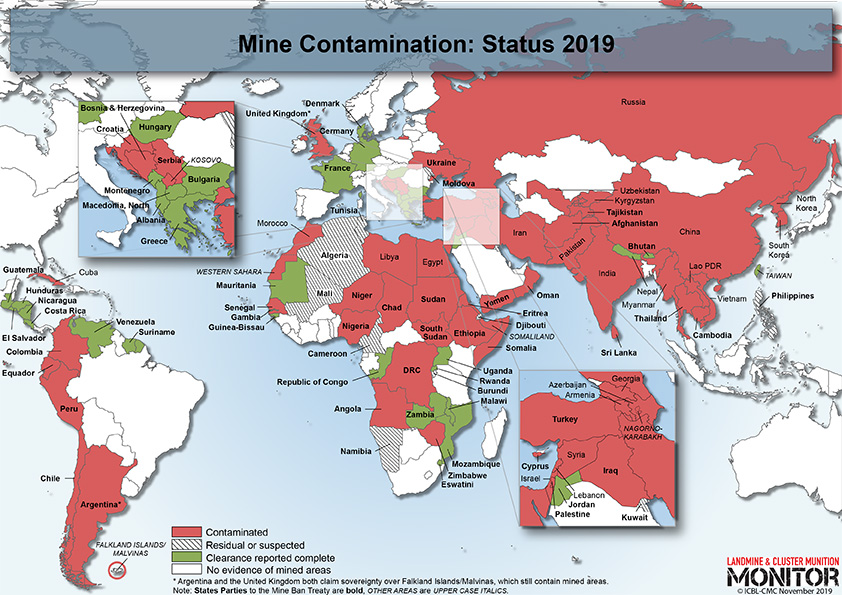
\includegraphics[width=\textwidth]{00 - Images/2019_MBT_Contamination_Final_Full.jpg}
  \caption{Worldwide contamination of landmines/\gls{erw} (2019) \cite{Monitor-Maps:online}}
  \label{fig:contamination_mine_erw}
\end{figure}

\section{Project code}

\subsection[language=C++]{main.cpp}

\lstinputlisting{../rpws/src/project_ros/src/main.cpp}

\subsection[language=C++]{ProjectRosMovement.cpp}

\lstinputlisting{../rpws/src/project_ros/src/ProjectRosMovement.cpp}

\subsection[language=C++]{ProjectRosTestSubscriber.cpp}

\lstinputlisting{../rpws/src/project_ros/src/ProjectRosTestSubscriber.cpp}
%%%%%

\end{document}